%----------------------------------------------------------------------------
\appendix
%----------------------------------------------------------------------------
\chapter*{\fuggelek}\addcontentsline{toc}{chapter}{\fuggelek}
\setcounter{chapter}{\appendixnumber}
%\setcounter{equation}{0} % a fofejezet-szamlalo az angol ABC 6. betuje (F) lesz
\numberwithin{equation}{section}
\numberwithin{figure}{section}
\numberwithin{lstlisting}{section}
%\numberwithin{tabular}{section}

%----------------------------------------------------------------------------
\section{A Bambu Slicer beállításai}
%----------------------------------------------------------------------------

\begin{figure}[h!]
	\centering
	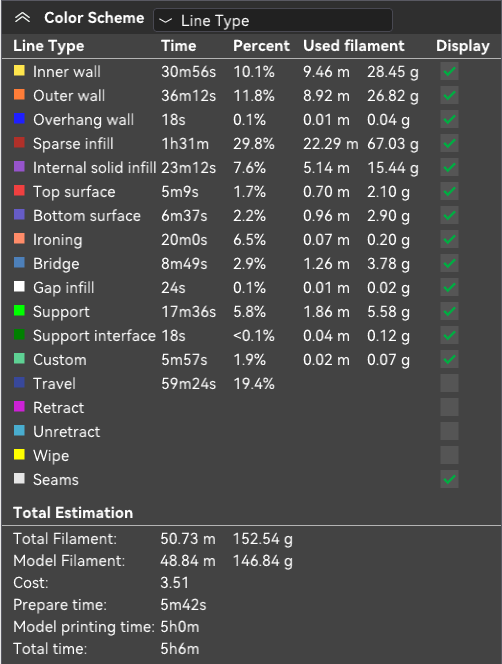
\includegraphics[width=0.7\linewidth]{fugg_slicer1}
	\caption{A Bambu Studio által szolgáltatott adatok}
	
\end{figure}

\begin{figure}[h!]
	\centering
	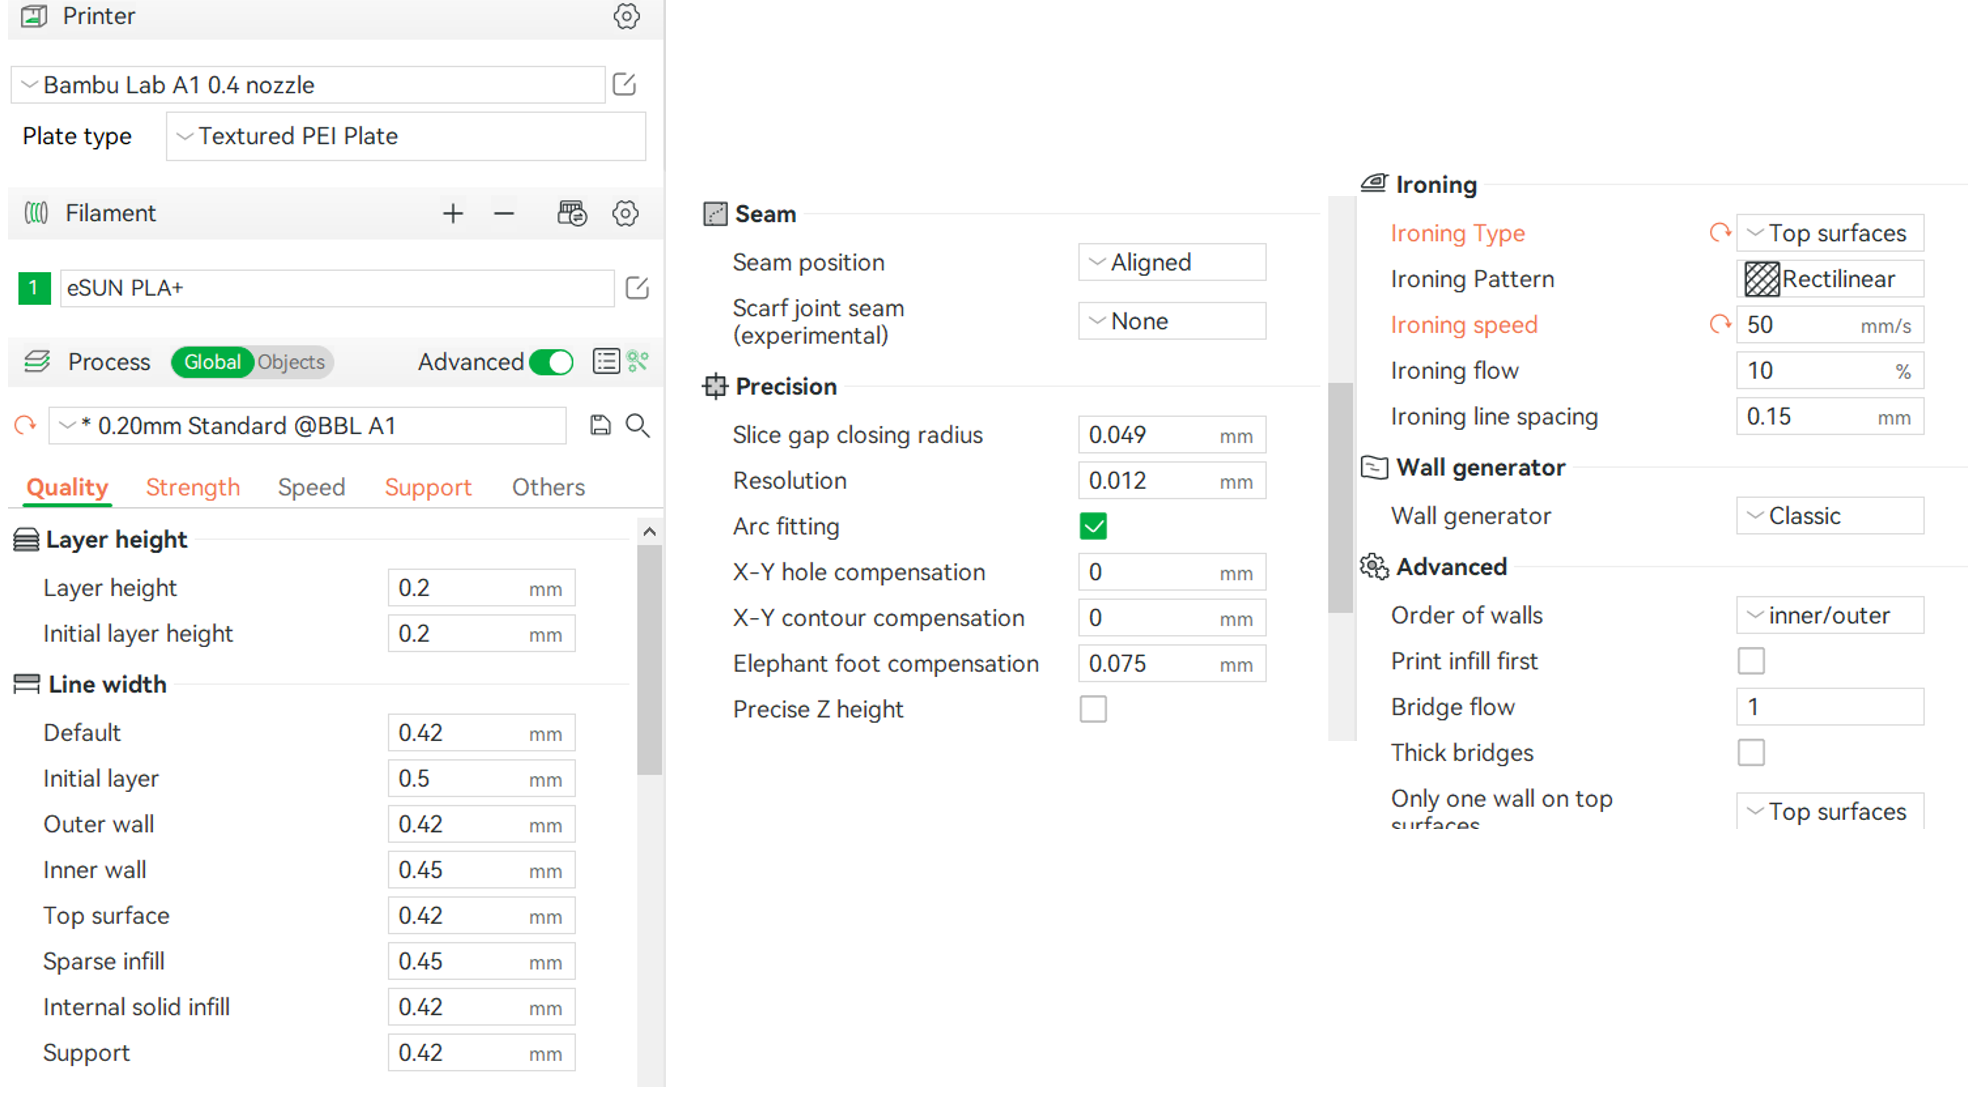
\includegraphics[width=1\linewidth]{fugg_slicer2}
	\caption{A Bambu Studio minőségi beállításai}
\end{figure}


\begin{figure}[h!]
	\centering
	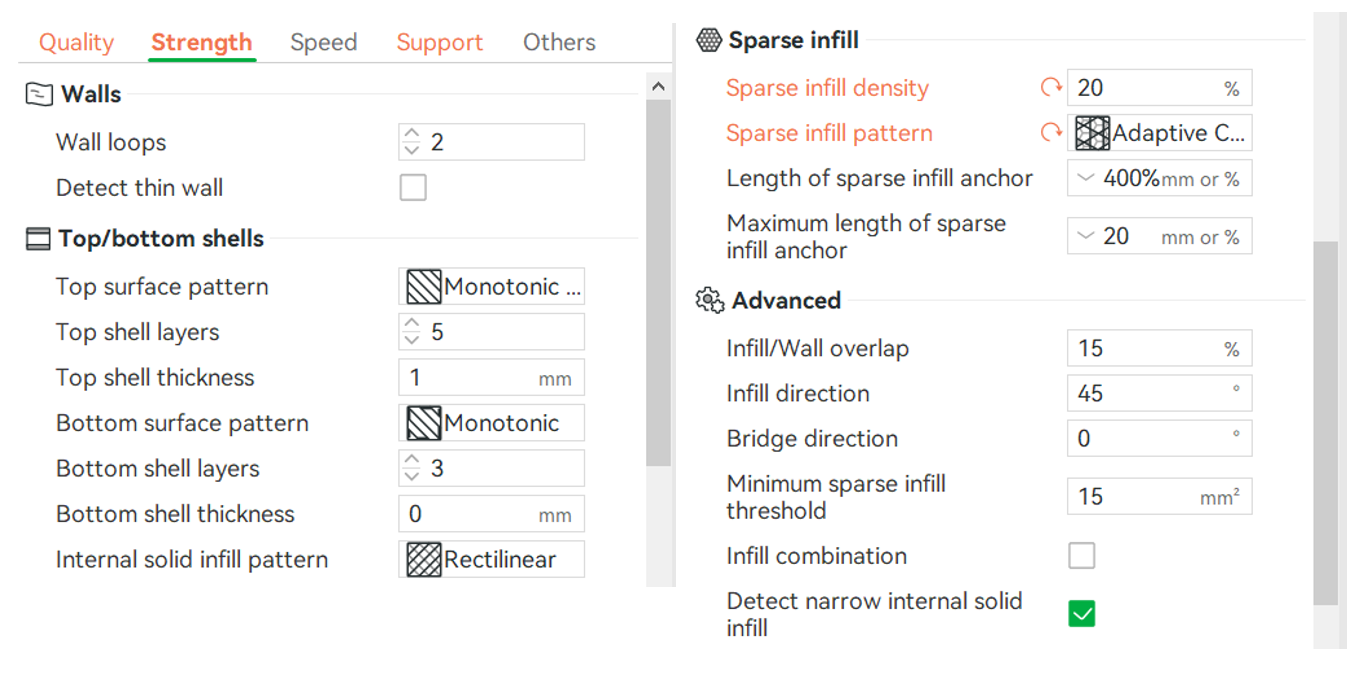
\includegraphics[width=1\linewidth]{fugg_slicer3}
	\caption{A Bambu Studio erősségi beállításai}
\end{figure}

\begin{figure}[h!]
	\centering
	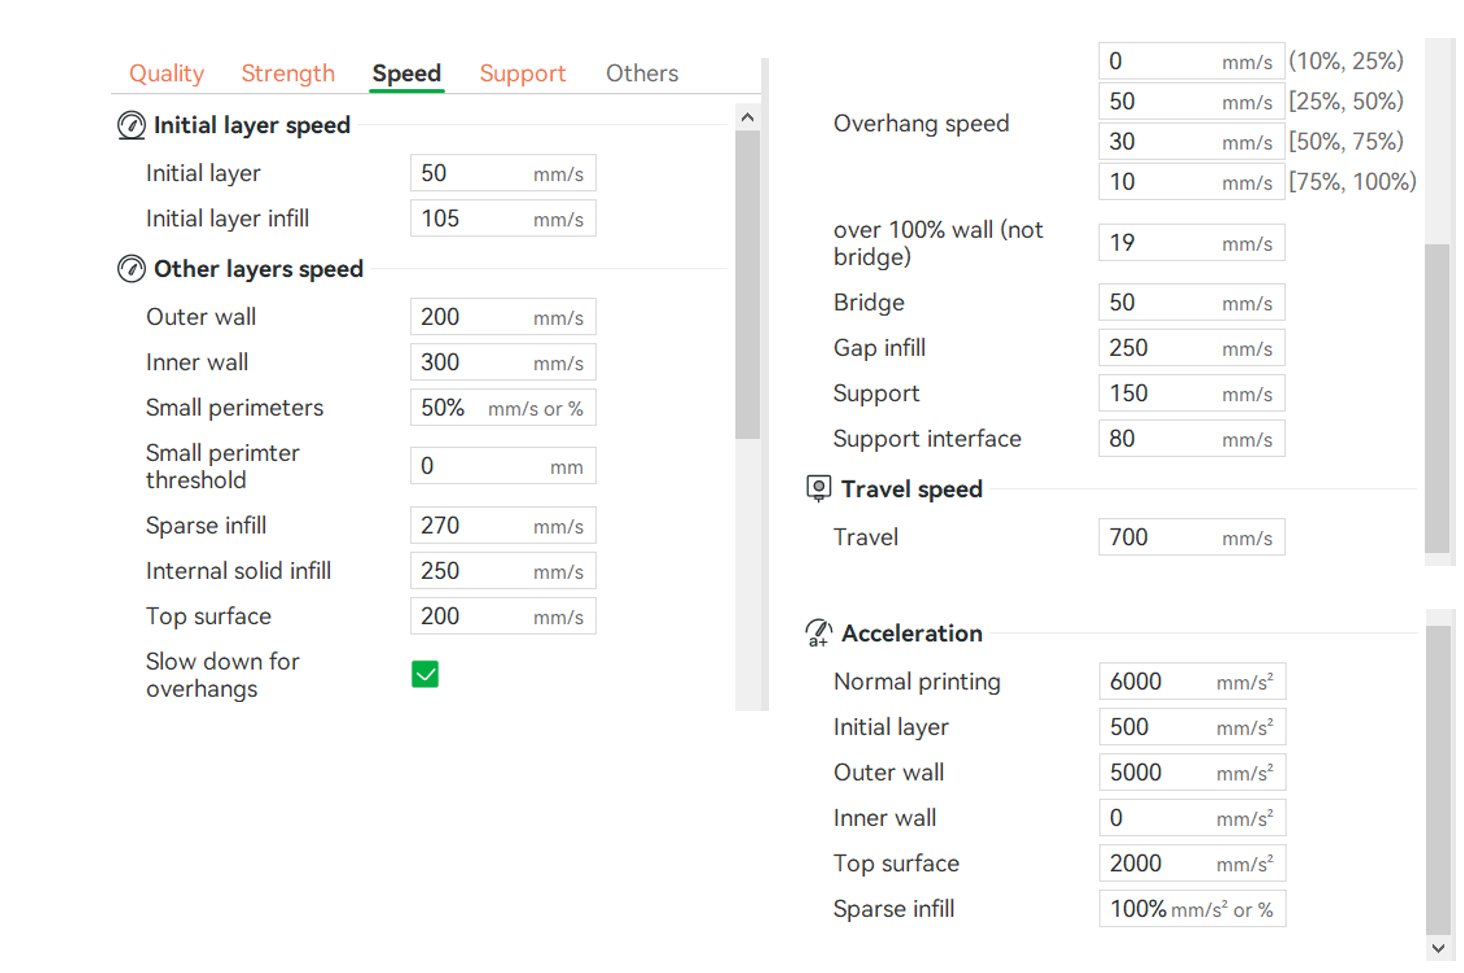
\includegraphics[width=1\linewidth]{fugg_slicer4}
	\caption{A Bambu Studio sebesség beállításai}
	
\end{figure}

\begin{figure}[h!]
	\centering
	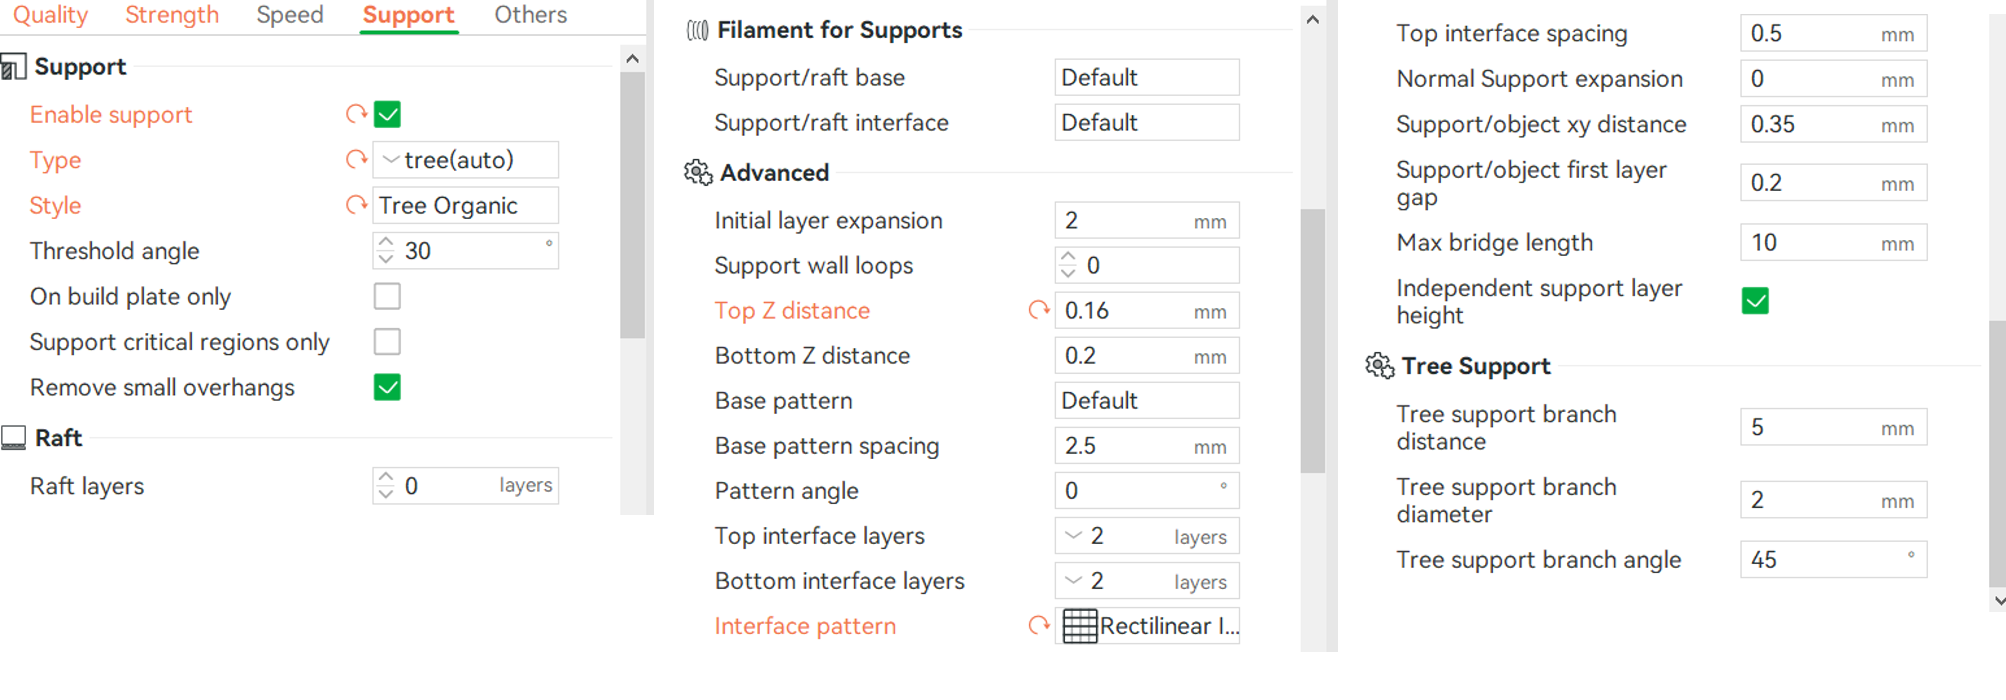
\includegraphics[width=1\linewidth]{fugg_slicer5}
	\caption{A Bambu Studio támasz beállításai}
	
\end{figure}